\subsubsection{Introduction}
The drug discovery process is mainly concerned with finding small molecules that interact with a target and have a therapeutic effect. However, a large source of failure in these endeavours has been the undruggability of targets.\cite{sMD_druggability} In these cases typical drug-like molecules cannot be used for various reasons, such as due to the shape (or absence) of the target pocket (e.g. in case of protein-protein interactions)\cite{sMD_scott-ppi-2016} or the nature of the active site (e.g. if it is highly charged).\cite{sMD_ptp-rev-druggability} An alternative to directly targeting the active site is allosteric inhibition, which is a way of affecting enzyme function at one site through binding at a different one, through a network of residue interactions \cite{sMD_Motlagh-allostery,sMD_Verkhivker-allostery} This allows the choice of pockets more suitable for small molecule drug design.

An example undruggable target is protein tyrosine phosphatase 1B (PTP1B), which has a charged active site. It is a negative regulator of insulin signalling\cite{sMD_ptp1b-diabetes} and is an attractive target for type II diabetes.\cite{sMD_Wiesman} The function of PTP1B depends on the conformation of its WPD loop, which can be closed (active) or open (inactive) (Figure \ref{fig:ptp1b}). It will be used as an example system for this tutorial.

\begin{figure}[htp]
\includegraphics[width=\linewidth]{03_steered_md/figures/open-close.png}
\caption{The WPD loop of PTP1B, in two conformations: open (yellow, PDB ID: 2HNP) and closed (red, PDB ID: 1SUG).}
\label{fig:ptp1b}
\end{figure}

Since allosteric inhibition is more complex than just physically blocking the active site, knowledge of good binding is not sufficient. An assessment of whether the binder is affecting protein function is required as well. One way of evaluating this is through populations of active and inactive conformations. Here this is achieved through Markov State Models (MSMs). \cite{sMD_Prinz} An MSM is an \textit{n $\times$ n} transition matrix that described the probability of the system transitioning to some state \textit{j} given that it is in state \textit{i}, after a given lag time $\tau$. The system is treated as memoryless, i.e. the transition probabilities do not depend on any previous states, only the current one.\cite{sMD_Husic-msm} This means model building only requires local equilibrium and can make use of multiple shorter trajectories. MSMs can thus model longer timescales without the associated computational cost.\cite{sMD_Prinz}

For the MSMs to more accurately represent statistical ensemble of protein configurations, enhanced sampling methods may be used. Steered molecular dynamics (sMD) is the focus of this tutorial. The WPD loop of PTP1B opens and closes on a $\mu$s timescale,\cite{sMD_Choy-Timescales} and therefore this transition is not observed on conventional computational timescales. sMD introduces a bias potential that is added to the Hamiltonian, thus biasing the simulation towards a specified value of a chosen collective variable (CV). This can be done via PLUMED, which is integrated in BioSimSpace.\cite{sMD_steeredMD,sMD_plumed-2} Once a larger conformational space has been explored via sMD, snapshots of various conformations can be used as starting points for equilibrium MD simulations. The trajectory data from those is then used to build an MSM (Figure \ref{fig:ensemble-protocol}).

\begin{figure}[htp]
\includegraphics[width=\linewidth]{03_steered_md/figures/ensemble-md-protocol.png}
\caption{The steps of using enhanced sampling methods to gather data for statistical analysis of protein conformation ensemble. (1) Run steered MD along some collective variable (CV); (2) Extract snapshots that evenly sample available conformational space; (3) Run equilibrium MD simulations using extracted coordinates as seeds; (4) construct an MSM using trajectory data from step 3.}
\label{fig:ensemble-protocol}
\end{figure}

\subsubsection{Running sMD using BioSimSpace}
sMD using BioSimSpace is very similar to regular production, starting with importing it and reading a parameterised and equilibrated system:
\begin{python}
import BioSimSpace as BSS
system = BSS.IO.readMolecules(["data/system.prm7", 
                                "data/system.rst7"])
\end{python}

The main requirement for sMD is to set up the CV. In this case, RMSD of all heavy atoms for residues of the WPD loop (179-185) will be used. For this, a reference structure is needed, as well as specific atom indices to be used for RMSD calculation:
\begin{python}
reference = BSS.IO.readMolecules("data/reference.pdb")
            .getMolecule(0)
rmsd_indices = []
for residue in reference.getResidues():
    if 178<=residue.index()<=184:
        for atom in residue.getAtoms():
            if atom.element()!="Hydrogen (H, 1)":
                rmsd_indices.append(atom.index())
rmsd_cv = BSS.Metadynamics.CollectiveVariable.RMSD(
                system, reference, 0, rmsd_indices)
\end{python}

One thing to note when dealing with RMSD between two different structures, is that the atoms may not be in the same order. For example, atom 1 in system in this case is a hydrogen, whereas in reference it is an oxygen. BioSimSpace takes care of this by matching up the atoms in the system to the atoms in the reference. The requirements for the reference structure are that all atoms found in reference.pdb must also exist in system. They are matched by residue number and atom name. For example, if the reference structure has an atom named CA in residue 1, there must be an equivalent in the system, and they will be mapped together.

BioSimSpace has a separate protocol for steering. To set one up, steering intervals and restraints need to be specified. Generally sMD consists of four stages (Table \ref{sMD-structure}). The end times of these stages are set:
\begin{python}
start = 0* BSS.Units.Time.nanosecond
apply_force = 4 * BSS.Units.Time.picosecond
steer = 150 * BSS.Units.Time.nanosecond
relax = 152 * BSS.Units.Time.nanosecond
\end{python}

\begin{table}
    \caption{sMD structure. Initially, the force is applied over a few picoseconds, followed by the steering (the bulk of the simulation). The force is removed at the end for system relaxation.}
    \label{sMD-structure}
    \begin{tabular}{|c|c|c|}
    \hline
       Stage  &  CV value  &  Force  \\
       \hline
        1. start  &  initial value  &  none \\
        \hline
        2. apply force  &  initial value  &  specified force  \\
        \hline
        3. steering  &  specified value  &  specified force  \\
        \hline
        4. relaxation  &  specified value  & none  \\
        \hline
    \end{tabular}
\end{table}

The length of the steering step is the most important here and will depend on the system, the steering force constant, and the magnitude of the change sMD is supposed to accomplish. The restraints specify the expected end CV values and the force constant ($\vec{s}_0$(t) and $\kappa$(t)) at each step created above. The protocol can then be created:
\begin{python}
nm = BSS.Units.Length.nanometer
restraint_1 = BSS.Metadynamics.Restraint(
                rmsd_cv.getInitialValue(), 0)
restraint_2 = BSS.Metadynamics.Restraint(
                rmsd_cv.getInitialValue(), 3500)
restraint_3 = BSS.Metadynamics.Restraint(0*nm, 3500)
restraint_4 = BSS.Metadynamics.Restraint(0*nm, 0)
protocol = BSS.Protocol.Steering(rmsd_cv, 
        [start, apply_force, steer, relax], 
        [restraint_1, restraint_2, restraint_3, restraint_4], 
        runtime=152*BSS.Units.Time.nanosecond)
\end{python}

This protocol can be used to create a process. At the moment sMD in BioSimSpace is supported with AMBER and GROMACS, and requires an installation of either of these MD engines patched with PLUMED.
\begin{python}
process = BSS.Process.Amber(system, protocol)
process.getConfig()
\end{python}
\begin{lstlisting}[columns=flexible]
['Production.',
 ' &cntrl',
...
 '  pres0=1.01325,',
 '  plumed=1,',
 '  plumedfile="plumed.dat,',
 ' /']
\end{lstlisting}

The lines plumed=1 and plumedfile="plumed.dat" are what specify that PLUMED will be used. The process can now be started to run steered MD.

\subsubsection{sMD trajectory analysis and seeded MD}
The sMD increases the number of starting conformations available for the MSM data. The next step is to save frames with various WPD loop conformations and use those as starting points for seeded MD simulations. As the sMD simulation is run, the CV values are saved to a \textbf{COLVAR} file. It can be plotted to assess whether the sMD simulation has been successful. An example is shown in Figure \ref{fig:rmsd}.

\begin{figure}[htp]
    \centering
    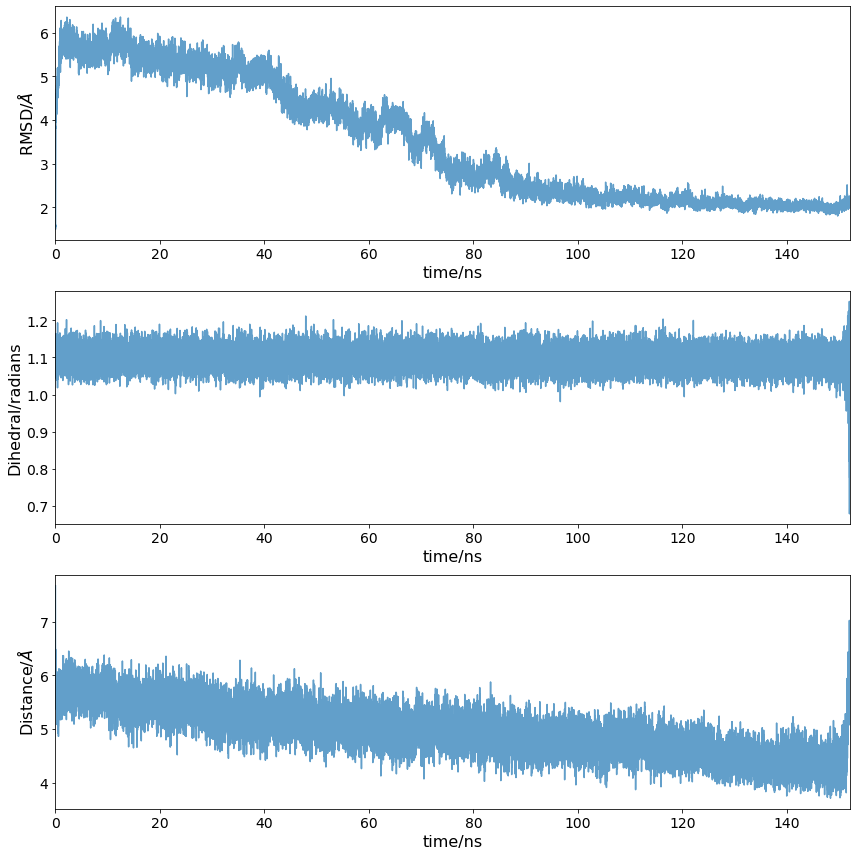
\includegraphics[width=\linewidth]{03_steered_md/figures/COLVAR_all.png}
    \caption{RMSD change throughout an sMD simulation. As the simulation progresses, the WPD loop RMSD gets closer and closer to the closed loop crystal structure (i.e. the loop is being closed).}
    \label{fig:rmsd}
\end{figure}

Once suitable frames have been chosen (here 100 evenly spaces snapshots are used as they sample the entire RMSD range), they can be saved as PDBs with BioSimSpace:
\begin{python}
for i, index in enumerate(frames):
    frame = BSS.Trajectory.getFrame(
    trajectory='/home/user/Documents/PTP1B/steering.nc', 
    topology = '/home/user/Documents/PTP1B/system.prm7', 
    index=int(index))
    BSS.IO.saveMolecules('data/snapshot_{i+1}',
                        frame, 'pdb')
\end{python}

These PDBs are then used as starting points for an array of 100 ns equilibrium MD simulations. As this requires a lot of computational resources, it is recommended to run this on an HPC cluster.

\subsubsection{Markov State Models}
There is a lot to consider when building MSMs, and the method is not covered in this tutorial. Here the python library \href{http://emma-project.org/latest/}{PyEMMA} was used, which has extensive examples and documentation. The exact method of building the following MSM is also provided in the jupyter notebook \textbf{03\_msm\_full.ipynb}.

The results of the data obtained from the results described above is shown in Figure \ref{fig:msm}. sMD was used to steer the WPD loop of PTP1B from open to closed and from closed to open, and 100 snapshots were extracted from each trajectory (200 in total). These were then used as starting points for 100 ns equilibrium MD simulations. The model indicates that this particular way of modelling PTP1B with peptide substrate results in catalytically active conformations 2\% of the time. Returning to the idea of allosteric inhibition, if a second model, built for a system including an allosteric binder of interest, showed a decrease in active conformation probability, it would suggest that this binder has inhibition potential. 

\begin{figure}[htp]
    \centering
    \includegraphics[width=\linewidth]{03_steered_md/figures/msm_final.png}
    \caption{The population of three metastables states as predicted by the MSM.}
    \label{fig:msm}
\end{figure}